%%%%%%%%%%%%%%%%%%%%%%%%%%%%%%%%%%%%%%%%%
% ELEE	3720 Electromechanical Energy Conversion: Report template
% By Ratheesh Ravindran
%%%%%%%%%%%%%%%%%%%%%%%%%%%%%%%%%%%%%%%%%
\documentclass[12pt]{article}
\usepackage[english]{babel}
\usepackage[utf8x]{inputenc}
\usepackage{amsmath}
\usepackage{graphicx}
\graphicspath{{Images/}}
\usepackage[colorinlistoftodos]{todonotes}
\usepackage{hyperref}
\usepackage{listings}

%\usepackage{fancyhdr}
%\pagestyle{fancy}
\begin{document}
\begin{titlepage}
\newcommand{\HRule}{\rule{\linewidth}{0.1mm}} 
\center % Center everything on the page
 
%---------------------------------------------------------------------------------
%	HEADING SECTIONS (Enter the Homework/assignment No., only)
%---------------------------------------------------------------------------------
\textsc{\Large Middle East Technical University}\\[0.5cm] % heading course Number
\textsc{\Large Department of Computer Engineering}\\[0.5cm] % heading course name
%\textsc{\large Homework/Assignment No:- }\\[0.5cm] % Minor heading
%---------------------------------------------------------------------------------
%	TITLE SECTION (Replace 'TITLE' with the Homework/assignment Name/title)
%---------------------------------------------------------------------------------

\HRule \\[0.4cm]
{ \huge CENG300}\\[0.3cm]
{ \huge SUMMER PRACTICE REPORT}\\[0.1cm] % Title of your Homework/assignment
%\HRule \\[1.5cm]
 
 \textsc{JotForm Yazılım A.Ş.}\\[0.1cm]
 \textsc{Hacettepe Teknokent Safir Bloklar C Blok Kat:6}
 \HRule \\[1.5cm]
 
%---------------------------------------------------------------------------------
%	AUTHOR SECTION (EDIT THE NAME and T.NO., only)
%---------------------------------------------------------------------------------

\begin{minipage}{0.4\textwidth}
\begin{flushleft} \large

\emph{Student's Name:}\\
Ozan \textsc{Şan}\\  % Enter Your name and T.No.
\end{flushleft}
%\begin{flushleft} \large

%\emph{Author 2:}\\
%Amna \textsc{Author-2}\\ T.No.  % Enter Your name and T.No.
%\end{flushleft}


\end{minipage}
\begin{minipage}{0.4\textwidth}
\begin{flushright} \large
\emph{Instructor:} \\
Prof.Dr.Göktürk Üçoluk% \textsc{Üçoluk} % Supervisor's Name
\end{flushright}
\end{minipage}\\[1cm]
{\large \today}\\[1cm] % Date, change the \today to a set date if you want to be precise

\includegraphics{cmetusmallest.png}\\[1.0cm]% \\[0.5cm] % 
%\vfill % Fill the rest of the page with white-space
Start Date: 10.06.2019 \\
End Date: 22.07.2019 \\
Total Working Days: 30 \\[1.2cm]
Student's Signature \hspace{150px} Organization Approval \\
\end{titlepage}
%%
% GradingRubric.tex
% This page will be the 2nd page of your report and will be used for grading the homework/assignment.
\section*{Grading Rubric - Information to Students}

Grading rubric that will broadly apply to assessing performance. That is, assessment exercises that are associated with a predominantly qualitative rather than quantitative character. If, for a particular exercise, there is substantial deviation from the scheme outlined below, I will let you know! Note: Be aware that if your “Quality of Presentation” is poor, it could impact scores assigned for the other two categories! (DO NOT EDIT THIS PAGE)
%\hspace*{-1.5in}
\begin{figure}[ht!]
    \centering
    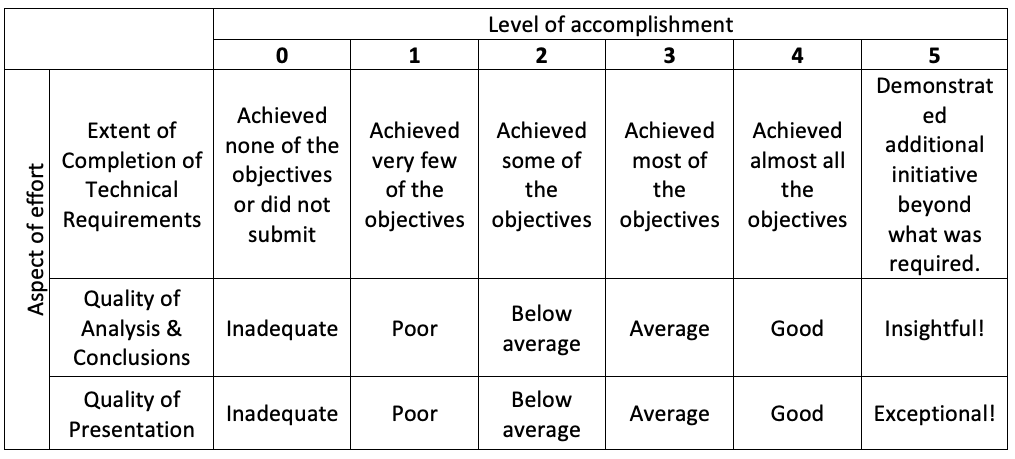
\includegraphics[scale=0.450]{LevelOfAccomplishments.png}
    \caption{Level of accomplishments}
    \label{fig:Level of accomplishments}
\end{figure}
\begin{table}[h]
    \centering
    \begin{tabular}{|c|c|}
    \hline
        Level &  Score \\
        \hline
        \hline
        5 &  12 (bonus!) \\
        \hline
        4: (`A`) &  10 \\
        \hline
        3: (`B`) &  8 \\
        \hline
        2: (`C`) &  6 \\
        \hline
        1: (`D`) &  4 \\
        \hline
        0: (`F`) &  0-2 \\
        \hline
    \end{tabular}
    \caption{Mapping of “Level” to “Score”}
    \label{tab:Mapping}
\end{table}
\begin{itemize}
    \item \textbf{Student's Level/Score (To be entered by Professor/GTA):}
\end{itemize}



\tableofcontents          % Required
%\listoffigures
%\listoftables
\newpage

% Do not edit the below sections, enter all details in respective chapters
% Add the images/screen-shorts to the image folder and insert them in the respective chapters

\section{Introduction}

% Introduction

I have completed my internship at JotForm Yazılım A.Ş., R\&D office, at Hacettepe Teknokent, Ankara. \\
My internship was about Time Series Analysis (TSA), and an implementation of a prediction system,
using metrics provided by JotForm. The metrics are numerical, and represents the state (mainly, financial state)
of the company. Using SARIMAX modelling, I have made a system which makes predictions about the future,
and, when in need, can be exported as a graph, and be further evaluated by the Data Science team of JotForm. This
will be further explained in further sections of this document.


\section{About JotForm Inc.}
JotForm is an international company, having offices in San Francisco, Izmir, and Ankara. Managerial
staff is primarily located in Ankara office, which is also the home for the main R\&D hub for the company. \\
\begin{figure}[hbt!]
    \centering
    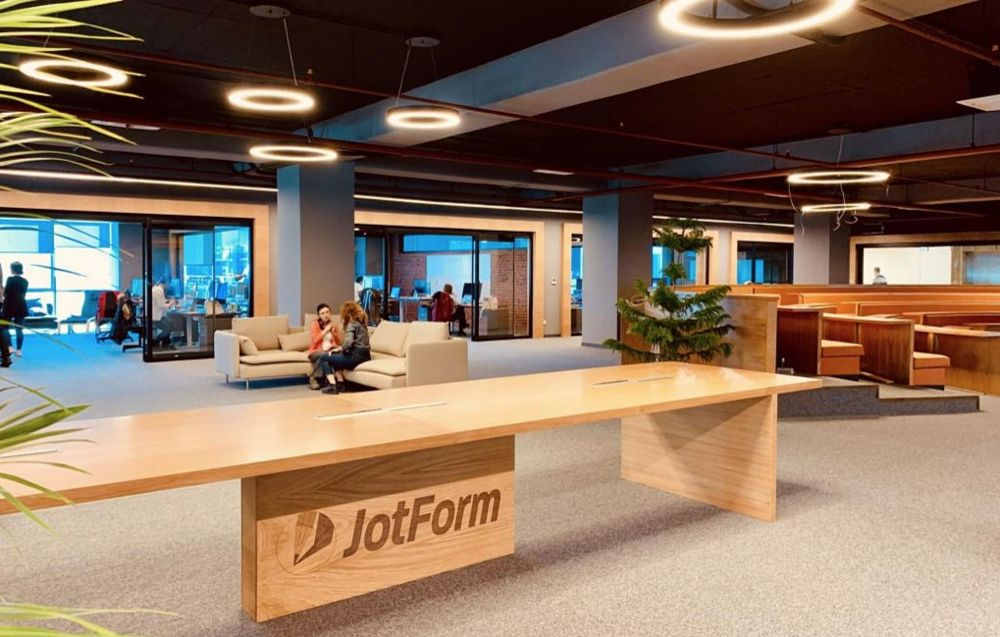
\includegraphics[width=0.9\textwidth]{Images/new-turkey-office.jpg}
    \caption{A View From JotForm's Ankara Offices}
    \label{fig:JFMAnkara}
\end{figure} \\
\subsection{Structure of the company}
In JotForm, employees are operating in teams, named by themselves, such as Amplify, Hermes and so on. The main responsibility of a team is not divided between different products of the company. This way, they can keep their focus, and work more reliably as a team. A team, for example, may work on Form Builder for a certain amount of time, and not in other products such as PDF Editor. This allows for an efficitent \textbf{Agile} work environment. \\
On fridays, all teams from Izmir and Ankara offices of JotForm come together for a meet, called the Demo Day. This facilitates for the presentations of the work done in the week for each team. This day is also the day for us interns to perform their presentations about their projects.

\subsection{Products offered by JotForm}
\subsubsection{Form Builder}
Form Builder tool is the main product of the company. Offering a drag-and-drop interface for creating forms,
analyzing data easily and making the analysis of the results from the form easier (using JotForm Sheets) is the main focus of the company. Since 2006, the founding of the company, they operate a Form Builder interface, which is active to this day. Main differences from competitors such as Google Sheets is the ease of use, and options for payment such as PayPal, Stripe etc. , which makes the product a standalone candidate for e-commerce websites, handling payments and billing information all by itself.

\subsubsection{PDF Editor}
In the last year, JotForm offices in Ankara started a project on PDF documents. Since the main focus of the company is on the forms, and customers repeatedly reporting that they need to convert their PDF forms to some online form, a team in Ankara office has built a tool for the purpose. In PDF editor, users can upload their fill-able PDF forms, and automatically transform them into an online form, hosted on JotForm. This feature also works in the other way around, as in, a user can take an existing online form in JotForm, and turn it into a fill-able PDF file format.

\subsubsection{JotForm Sheets}
Primarily to relieve their customers from needing to resort to Google's services, mainly, Google Sheets, the company developed a tool to deal with Spreadsheet files.
This is integrated into their form builder environment, so that the customers can perform aggregate functions similar to Microsoft Excel™, analyze large amount of responses to their forms, and export to useful file formats, such as .csv files.

\section{Project}
The project I have completed is called JFM Overseer. Overseer is an application written in Python 3.7, preferably for use with Anaconda distributions, and is capable of predicting time series. The overall structure of the application is as in the following diagram: \\
\begin{table}[ht]
\centering
\begin{tabular}{|l|ll} 
\cline{1-1}\cline{3-3}
GUI components (PyQT5) & \multicolumn{1}{l|}{$\rightarrow$} & \multicolumn{1}{l|}{Matplotlib}  \\ 
\cline{1-1}\cline{3-3}
Facebook Prophet \& StatsModels  &                         &                        \\ 
\cline{1-1}
Pandas  &                         &                        \\ 
\cline{1-1}
Time Series Data (.csv)  &                         &                        \\
\cline{1-1}
\end{tabular}
\end{table} \\
The components and how to set them up are as follows:
\subsection{Time Series Data Specifications}
Overseer is a tool to analyze Time Series data, which must be given to the program as .csv files, with the following structure: \\

\begin{table}[ht]
\centering
\begin{tabular}{| l | l |}
$ds$    & $y$    \\
$t_0$  & $y_0$  \\
\vdots & \vdots
\end{tabular}
\end{table}
In this representation, $t$ must correspond to a date-time value, mainly, parse-able by Matplotlib and other software used. The values for y must be integers. \\
This lets us create a function $F(t) = y$, which is useful in upcoming definitions.
My goal was mainly to produce a prediction, namely, we have to define values $m_t, n_t$ such that for any $t > t_{end}$, where the last observed point of the function F is at time $t_0 + end$, the equation
\begin{equation*}
	P(m_{t} < F(t) < n_{t}) = 0.95
\end{equation*}

must hold. This corresponds to creating a $95\%$ probability interval for the possible observed values of the function $F$ in the future, and means that we have made a prediction. The values $m_t$ and $n_t$ can be averaged to yield a possible future value of $F$. The process for doing this was explained in (Box and Wilkins CITE). However, before getting to that, we must first process the data. 

\subsection{Pandas}
Pandas is a tool to analyze spreadsheets, and process them in Python, dubbed ``Excel for Python". It has capabilities in displaying, analyzing, converting and processing data.
\subsubsection{How To Install}
In a shell, execute:

\begin{lstlisting}[language=bash]
pip install pandas
\end{lstlisting}
... or, in an Anaconda environment, use:
\begin{lstlisting}[language=bash]
conda install pandas
\end{lstlisting}
to install Pandas to your preferred Python environment. Using Anaconda distributions is recommended for resolving dependency problems, as nearly all of the packages used in the project are already included in Anaconda distributions.
\subsubsection{Usage}
An example code snippet from the project is as such:
\begin{lstlisting}[language=Python]
import pandas as pd
df = pd.read_csv(data.csv)
\end{lstlisting}
This loads the .csv file into memory, and is modified to suit our needs as such (will be further explained in (XREF FBPROPHET)):
\begin{lstlisting}[language=Python]
#'COL1' denoting the first column's name
# in the .csv file, this was primarily
# called 'Category' in my company's query results.
df['COL1'] = df['COL1'].apply(pd.to_datetime)
dataframe.columns = ['ds', 'y']
\end{lstlisting}
After doing this, we can work further on the data.

\section{Methodology}
% Methodology or Algorithm or Theoretical know-how or steps to run your code/simulations
% Please delete the below lines and enter details for this assignment/homework

    This section should be dedicated to explaining the 'theoretical know-how' or 'steps to run your code' or 'algorithms used'. 

The following are guidelines. Use your judgment appropriately

\begin{enumerate}
\item Explain your approach to solving this homework assignment (theoretical know-how)
\item Which concepts from the class did you apply in this homework?  How did you apply them? State the assumptions made, including the reason for assumptions.
\item Are there any special steps that should be followed to run/simulate your program/files on other computer, with necessary software (MATLAB/MULTISIM)?
\item Explain the main parts of your algorithm with the help of a flowchart, if appropriate. What does each section of it do? 
\end{enumerate}




 Note:
\begin{itemize}
\item  In MATLAB, Lines of comment embedded in the program are essential. However, comments cannot be used as a substitute for the algorithm explanations asked for above!
\item  Remember, these questions are just examples to guide you in explaining your methodology. You may not need to answer all of them in all homework assignments. You may need to add more information in a particular report. Use your judgment appropriately!
\end{itemize}




\section{Results}
% Results
% Please delete the below lines and enter details for this assignment/homework
\begin{itemize}
\item  The results obtained should be placed here. Attach the screen shots (with description labels) from your simulation to show the schematic circuit, static/transient response, other results, as per the homework/assignment. Also, if something unexpected happened (errors/issues), attach screen shot (with description labels). Use graphs when appropriate to demonstrate results. 
\end{itemize}

\section{Discussions and Conclusion}
% Discussions & Conclusion
% Please delete the below lines and enter details for this assignment/homework
    Finally, discuss your results and state your conclusions on the task you were given in this
homework.
\begin{enumerate}
\item Did you meet the goals of this homework?
\item What was the key elements of theoretical know-how taken into consideration ?
\item If there is any errors/issues, what do you think about this error/issue? How can you do to fix it?
\item If your simulation/calculation works mostly as expected, but fails in some scenarios, what do you think or state the possible reasons, try to propose a solution?
\item What are the limitations of your code/simulation?
\item Make a comment about how this homework affected your knowledge of the subject.
\end{enumerate}


\bibliographystyle{plain}
\bibliography{Bibliography.bib}

\appendix
\section{Appendix}
%
% Please attach the MATLAB or MULTISIM files (finial version) with this report
% Please delete the below lines and enter details for this assignment/homework
 Include your code here! \\
 
\textbf{ Note: Also ensure to attach the MATLAB or MULTISIM files with this report.}



%---------------------------------------------------------------------------------
%	Example SECTION (Remove this section to finalize the report.


\section{Example steps}
% These are some example steps 
% Refer https://www.overleaf.com/learn/how-to/Creating_a_document_in_Overleaf


\subsection{Sub Sections}

Use section and subsection commands to organize your document. \LaTeX{} handles all the formatting and numbering automatically. Use ref and label commands for cross-references.

\subsection{Comments}

Comments can be added to the margins of the document using the \todo{Here's a comment in the margin!} todo command, as shown in the example on the right. You can also add inline comments too:

\todo[inline, color=green!40]{This is an inline comment.}

\subsection{Tables and Figures}

Use the table and tabular commands for basic tables --- see Table~ \ref{tab:widgets}, for example. You can upload a figure (JPEG, PNG or PDF) using the files menu. To include it in your document, use the include graphics command as in the code for Figure~\ref{fig:Speed vs. Torque from Pittman} below.

\begin{table}[h]
\centering
\begin{tabular}{|l|r|}
\hline
Item & Quantity \\\hline
Widgets & 42 \\ \hline
Gadgets & 13 \\ \hline
\end{tabular}
\caption{\label{tab:widgets}An example table.}
\end{table}

% Commands to include a figure:
\begin{figure}[hbt!]
    \centering
    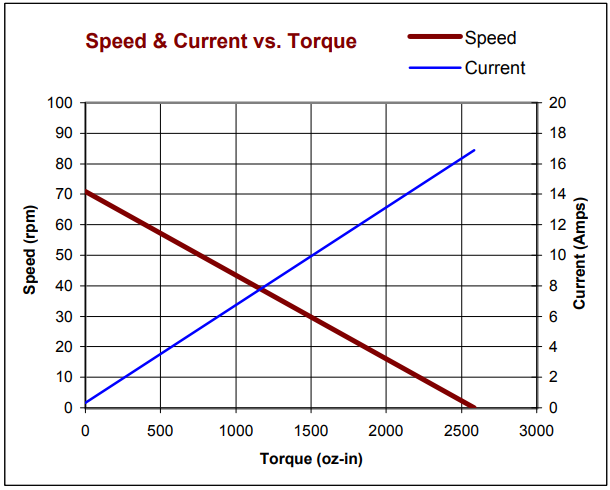
\includegraphics[width=0.9\textwidth]{Images/SpeedvsTorque.png}
    \caption{Speed vs. Torque from Pittman motor data sheet}
    \label{fig:Speed vs. Torque from Pittman}
\end{figure}





\subsection{Mathematics}

\LaTeX{} is great at typesetting mathematics. Let $X_1, X_2, \ldots, X_n$ be a sequence of independent and identically distributed random variables with $\text{E}[X_i] = \mu$ and $\text{Var}[X_i] = \sigma^2 < \infty$, and let
$$S_n = \frac{X_1 + X_2 + \cdots + X_n}{n}
      = \frac{1}{n}\sum_{i}^{n} X_i$$
denote their mean. Then as $n$ approaches infinity, the random variables $\sqrt{n}(S_n - \mu)$ converge in distribution to a normal $\mathcal{N}(0, \sigma^2)$.

\subsection{Lists}

You can make lists with automatic numbering \dots

\begin{enumerate}
\item Like this,
\item and like this.
\end{enumerate}
\dots or bullet points \dots
\begin{itemize}
\item Like this,
\item and like this.
\end{itemize}

%% cite an article
\subsection{Bibliography}
\begin{itemize}
    \item Adding bibliography to document
	\item Some claim \cite{gratzer2007more}.
\end{itemize}

\subsection{Hyperlink to a website}
%% Hyperlink to a website
\begin{itemize}
    \item \href{https://www.overleaf.com/latex/templates/a-quick-guide-to-latex/fghqpfgnxggz}{Hyperlink to a website}.
\end{itemize}



\subsection{Learn LaTeX in 30 minutes}
\begin{itemize}
    \item \href{https://www.overleaf.com/learn/latex/Learn_LaTeX_in_30_minutes}{Link to overleaf website}.
\end{itemize}

 % Remove this line to finalize the report.
%---------------------------------------------------------------------------------


\end{document}


% Note: Again, you don’t need to answer just the above questions. They are being provided to give you a flavor of what is required for each section. Use your judgment and initiative to add or subtract based on the specific homework. You can add any other conclusion or discuss any other aspect of your effort that you think it is important to highlight.

% Also ensure to attach the MATLAB or MULTISIM files with this report